\section{Model generalisation}

Fig.~\ref{fig:imm} illustrates a probabilistic graphical representation of the IMM.

\begin{figure}[htbp]
\centering
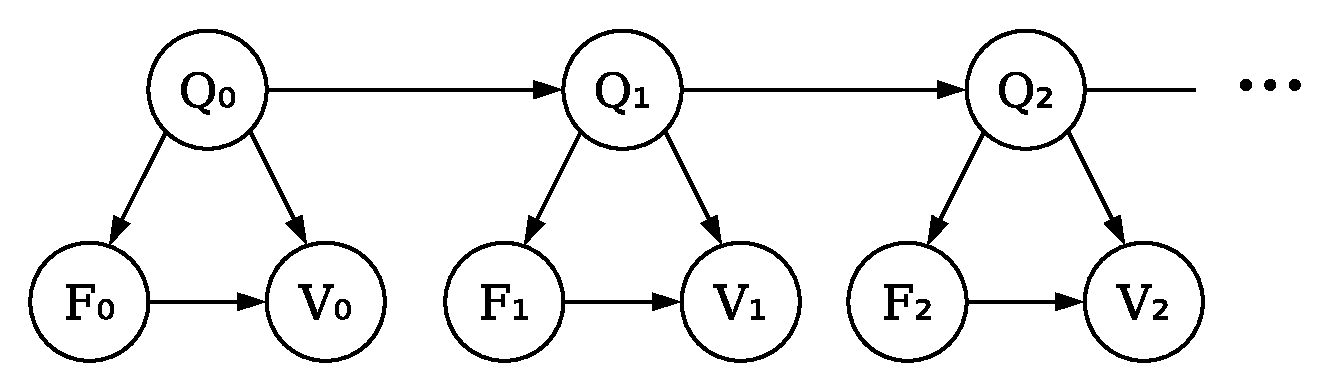
\includegraphics[width=.45\linewidth]{figure/imm}
\caption{Invisible Markov model.}%
\label{fig:imm}
\end{figure}


\newpage
\newpage

\section{Old model generalisation}

Let $L_t=F_0+F_1+\dots + F_{t-1}$ be the random variable describing the number of emitted symbols right
before the sequence emission by $Q_t$.
Let $S_1, S_2, \dots$ a stochastic process for symbol emission such that $S_t\in\set{A}$
and
\begin{align*}
    p(s_{l_t+1} .. s_{l_t+f_t}, L_t=l_t, F_t=f_t, V_t=\mathbf v_t)
        = p(s_{l_t+1} .. s_{l_t+f_t}\gv L_t=l_t, F_t=f_t, V_t=\mathbf v_t).
\end{align*}

Let us define an additional stochastic process  associated with a given IMM
(random variables are omitted for didactic reasons whenever appropriate):
\begin{align*}
    p(S_0=\emptyset\gv Q_0=q_0)
        &=1\\
    p(s_1 .. s_{f_1},f_1,q_1)
        &= p(s_1 .. s_{f_1}\gv f_1,q_1)p(f_1,q_1) = p(s_1 .. s_{f_1}\gv f_1,q_1)p(f_1\gv q_1)p(q_1)\\
    p(s_1 .. s_{f_1+f_2},f_1,f_2,q_1,q_2)
        &= p(s_{f_1+1} .. s_{f_1+f_2}\gv f_1, f_2, q_2)p(s_1 .. s_{f_1}, f_1, f_2, q_1, q_2)\\
        &= p(s_{f_1+1} .. s_{f_1+f_2}\gv f_1, f_2, q_2)p(s_1 .. s_{f_1}\gv f_1, q_1) p(f_1, f_2, q_1, q_2)\\
        &= p(s_{f_1+1} .. s_{f_1+f_2}\gv f_1, f_2, q_2)p(s_1 .. s_{f_1}\gv f_1, q_1) p(f_1\gv q_1) p(f_2\gv q_2)p(q_2\gv q_1)p(q_1)
\end{align*}

\begin{figure}[htbp]
\centering
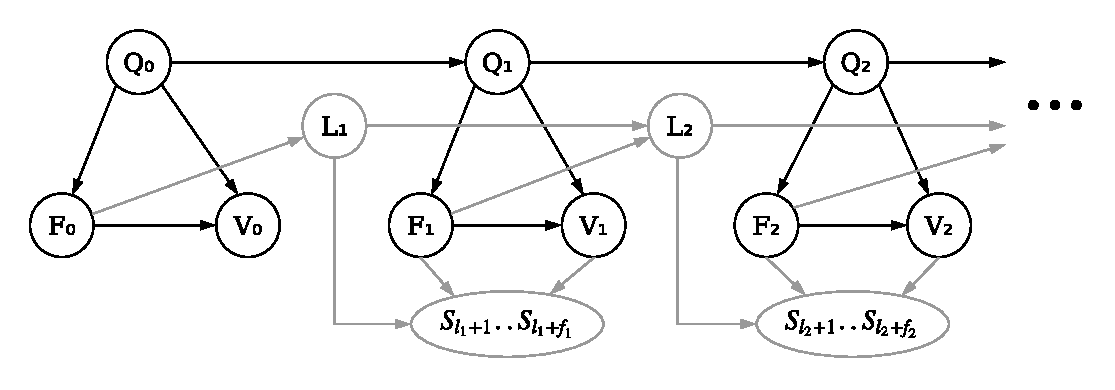
\includegraphics[width=.6\linewidth]{figure/imm-s}
\caption{Invisible Markov model with symbol emission stochastic process.}%
\label{fig:imm-s}
\end{figure}

Let $L_t=F_0+F_1+\dots + F_{t-1}$, be the random variable describing the number of emitted symbols right
before the sequence emission by $Q_t$.
We define
\begin{align*}
    p(S_{l_t+1}=s_{l_t+1}, \dots, S_{l_t+f_t}=s_{l_t+f_t} \gv L_t=l_t, F_t=f_t, Q_t=q_t) =
                                p(V_t=(s_{l_t+1}, \dots, s_{l_t+f_t}) \gv F_t=f_t, Q_t=q_t).
\end{align*}
Given an IMM, we define the marginal likelihood of a sequence $\mathbf z = z_1z_2\dots z_L$
as being
\begin{align*}
    p(S_1=z_1, \dots, S_L=z_L) = \sum\limits_{\substack{q_1..q_N \\ f_1..f_N}}
        p(S_1=z_1, \dots, S_L=z_L, Q_1=q_1, F_1=f_1, \dots, Q_N=q_N, F_N=f_N),
\end{align*}
subject to $L=l_N+f_N$.\footnote{It might be a good moment to talk about degenerate IMM: when there is silent states cycle and/or
there are states with unbounded sequence lengths.}

Silent and non-silent HMM states are particular cases of IMM states that emit sequences of length zero and one,
respectively.

% \begin{align*}
%     p(S_{i_t}=s_{i_t}, S_{i_t+1}=s_{i_t+1}, \dots, S_{i_t+f_t-1}=s_{i_t+f_t-1} &| I_t=i_t, F_t=f_t, Q_t=q_t) =\\
%                                             &p(V_t=(s_{i_t}, s_{i_t+1}, \dots, s_{i_t+f_t-1}) | F_t=f_t, Q_t=q_t).
% \end{align*}

% \section{Old model generalisation}

% The standard HMM description (Def.~\ref{def:hmm}) is usually extended to account for states that do not emit symbols.
% Those states are referred to as silent states and are useful to describe a missing alignment position, for example.
% This section goes a step further by defining an alternative Markov model that accounts for states that instead
% emit sequence of symbols of variable length.

% \begin{definition}
% Let $\set{A}$ be a finite set of symbols.
% Let $Q_1, Q_2, \dots$ be a Markov process and $F_1, F_2, \dots$ be a stochastic process for which
% \begin{equation*}
%     p(F_t\in\field{N}\gv Q_1=q_1, Q_2=q_2, \dots, Q_t=q_t) = p(F_t\in\field{N}\gv Q_t=q_t).
% \end{equation*}
% Let $V_1, V_2, \dots$ be a stochastic process for which
% \begin{equation*}
%     p(V_t\in\set{A}^{f_t}\gv Q_1=q_1, F_1=f_1, Q_2=q_2, F_2=f_2, \dots, Q_t=q_t, F_t=f_t)
%         = p(V_t\in\set{A}^{f_t}\gv Q_t=q_t, F_t=f_t).
% \end{equation*}
% The triplet $(Q_t, F_t, V_t)$ is an invisible Markov model (IMM) with alphabet $\set{A}$.
% \end{definition}

% Silent and non-silent states are particular cases of IMM states that emit sequences of length zero and one,
% respectively.
% IMM reduces to the standard HMM if $p(F_t=1\gv Q_t=q_t)$ for every $t$.
% Fig.~\ref{fig:imm} illustrates a probabilistic graphical model for IMM.

% Let us define an additional stochastic process $S_1, S_2, \dots$ associated with a given IMM as follows.
% Let $L_t=F_1+\dots + F_{t-1}$, for which $L_1 = 0$, be the random variable describing the number of emitted symbols right
% before the sequence emission by $Q_t$.
% We define
% \begin{align*}
%     p(S_{l_t+1}=s_{l_t+1}, \dots, S_{l_t+f_t}=s_{l_t+f_t} \gv L_t=l_t, F_t=f_t, Q_t=q_t) =
%                                 p(V_t=(s_{l_t+1}, \dots, s_{l_t+f_t}) \gv F_t=f_t, Q_t=q_t).
% \end{align*}
% Given an IMM, we define the marginal likelihood of a sequence $\mathbf z = z_1z_2\dots z_L$
% as being
% \begin{align*}
%     p(S_1=z_1, \dots, S_L=z_L) = \sum\limits_{\substack{q_1..q_N \\ f_1..f_N}}
%         p(S_1=z_1, \dots, S_L=z_L, Q_1=q_1, F_1=f_1, \dots, Q_N=q_N, F_N=f_N),
% \end{align*}
% subject to $L=l_N+f_N$.\footnote{It might be a good moment to talk about degenerate IMM: when there is silent states cycle and/or
% there are states with unbounded sequence lengths.}

\begin{sidewaysfigure}[ht]
    \centering
    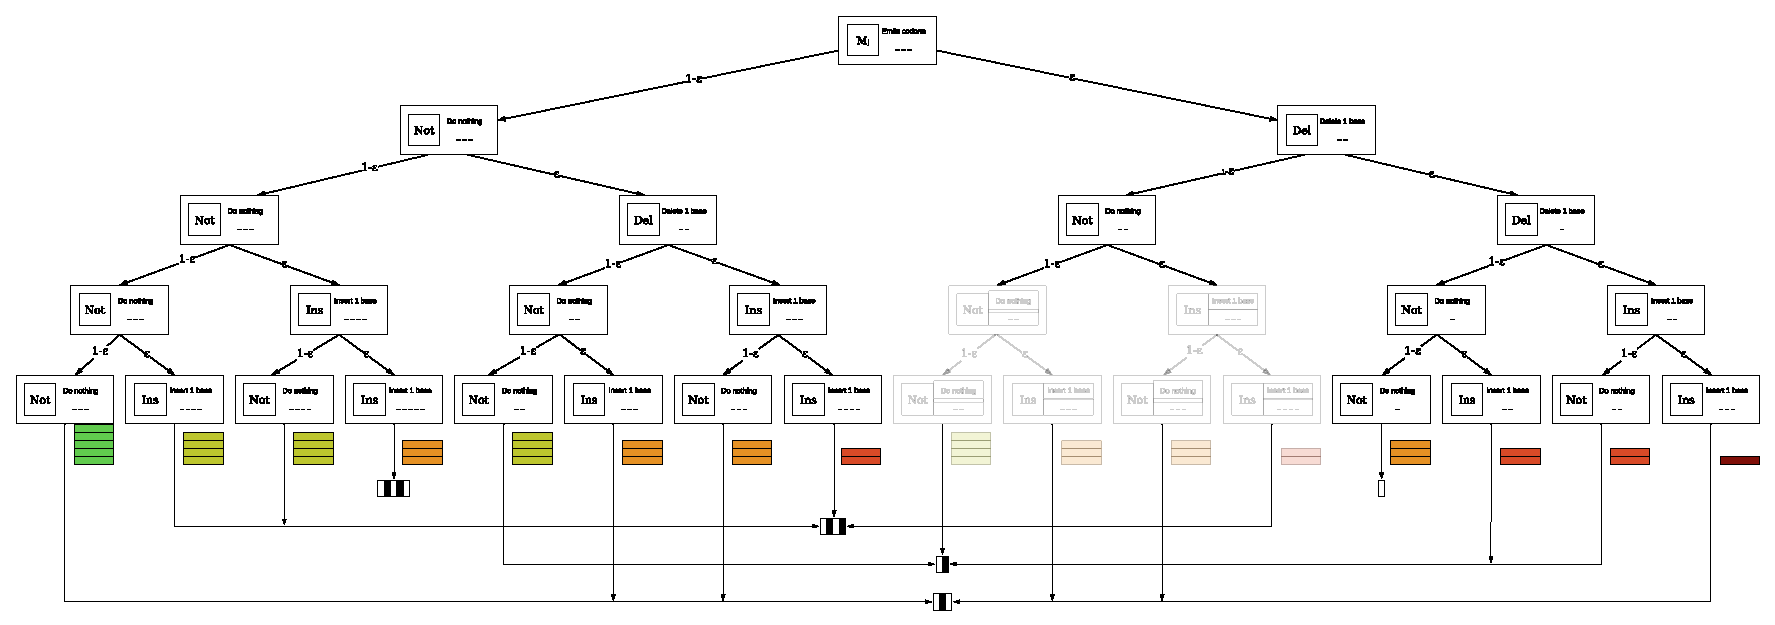
\includegraphics[scale=0.9]{figure/codon-hmm-tree}
    \caption{Matched codon HMM tree.
        The $\eps$-transitions occur infrequently and exist to account for sequence errors.
        The most probably path ends at the first leaf-node from left to right.}\label{fig:codon-hmm-tree}
\end{sidewaysfigure}

% Writting the marginal likelihood as in Eq. \eqref{eq:ml} is rather tedious.
% To alleviate this problem, let $F_t$ be the sequence length emitted by $S_t$,
% $L_t \eqdef 0+F_1+\dots+F_{t-1}$, and $S_{1..t} \eqdef S_1||S_2||\dots||S_t$.
% We have
% \begin{align*}
%   p(S_{1..1} \neq \arr{z}, S_{1..2} \neq \arr{z}, \dots, S_{1..{t-1}} \neq \arr{z}, S_{1..t}=\arr{z})
%   = p(S_{1..t}=\arr{z}, L_t<L).
% \end{align*}
% Therefore, the marginal likelihood is also given by
% \begin{align*}
%   \mathrm{ML}(\arr{z}) = \sum_{t=1}^{\infty} p(S_{1..t}=\arr{z}, L_t<L).
% \end{align*}
